\documentclass[12pt]{report}

\usepackage[russian]{babel}
\usepackage[utf8]{inputenc}
\usepackage{amsmath}
\usepackage{amssymb}
\usepackage{tikz}
\usepackage{caption}
\usepackage[a4paper,margin=1.0in,footskip=0.25in]{geometry}
\usepackage{listings}  
\usepackage{color}
\usepackage{tabto}
\usepackage{graphicx}

\definecolor{dkgreen}{rgb}{0,0.6,0}
\definecolor{gray}{rgb}{0.5,0.5,0.5}
\definecolor{mauve}{rgb}{0.58,0,0.82}

\lstset{frame=tb,
  language=Python,
  aboveskip=3mm,
  belowskip=3mm,
  showstringspaces=false,
  columns=flexible,
  basicstyle={\small\ttfamily},
  numbers=none,
  numberstyle=\tiny\color{gray},
  keywordstyle=\color{blue},
  commentstyle=\color{dkgreen},
  stringstyle=\color{mauve},
  breaklines=true,
  breakatwhitespace=true,
  tabsize=3,
  frame=none
}

%Title
\title{\vspace{-3cm}Лабораторная №7}
\author{Жидович Максим, группа №1}
\date{22 декабря 2021}

\renewcommand\thesection{\arabic{section}}

\begin{document}

\maketitle

\section{Постановка задачи}

\tabВычислить корни собственного многочлена четвертой степени $P(\lambda)$, полученного из
канонической формы Фробениуса лабораторной работы №5 «Метод Данилевского».
Произвести отделение корней многочлена $P(\lambda)$. Для определения промежутков
монотонности функции $P(\lambda)$ решить уравнение $P^{\prime}(\lambda) = 0$ методом простой итерации или методом Ньютона (на выбор). Предварительно произвести отделение корней многочлена
$P^{\prime}(\lambda) = 0$.


\section{Входные данные}

В работе использовались:

Матрица $A$ 4 порядка:
\[ 
\begin{bmatrix}
60 & 944 & 34483 & -5945475 \\
1 & 0 & 0 & 0\\
0 & 1 & 0 & 0 \\
0 & 0 & 1 & 0 \\
\end{bmatrix}
\]

Многочлен:
\[P(\lambda) = x^4 - 60 x^3 - 944 x^2 - 34483 x + 5945475\]

\section{Теория}

\tabПроведём отделение корней многочлена $P^{\prime}(\lambda)$. При отделении корней многочлена $P^{\prime}(\lambda)$ найдём промежутки монотонности функции $P^{\prime}(\lambda)$, решив квадратное уравнение $P^{\prime\prime}(\lambda) = 0$ Воспользуемся Wolfram:
\[
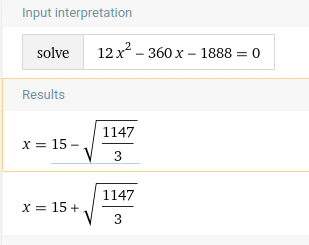
\includegraphics[scale=0.5]{roots_lab07_2d.png}
\]
\tabПроверим значения $P^\prime(\lambda)$ в этих точках, а так же в $-\infty$ и $+\infty$. В результате делаем вывод, что единственный вещественный корень $P^\prime(\lambda) = 0$ будет лежать в интервале $]15 + \sqrt{\frac{1147}{3}}; +\infty[$

Затем решим уравнение $P^\prime(\lambda) = 0$ с помощью метода Ньютона, выбрав в качестве начального приближения $15 + \sqrt{\frac{1147}{3}}$ и $\epsilon = 0.0001$.
\[
x = 56.1423
\]

Найдём значение $P(\lambda)$ в точке $x$:
\[
P(x) = 351420.3533
\]

$P(\lambda) > 0$, а значит многочлен не имеет действительных корней, имеет место случай 1:

$P(\lambda)$ не имеет вещественных некратных корней. Тогда, возможно, два наибольших по модулю корня образуют комплексно-сопряженную пару и имеет место Случай 4 файла
«Степенной метод». Получим собственные значения и соответствующие им собственные
векторы согласно теории Случая 4. 

\section{Листинг программы}

\lstset{language=Python}
\lstset{extendedchars=\true}

\begin{lstlisting}
 def f(p, x):
	"""Find p(x)"""
	result = 0
	n = len(p)
	for i in range(n):
		result += p[i] * (x**(n-i-1))

	return result


def f_diff(p, x):
	"""Find p`(x)"""
	p_copy = np.copy(p)
	
	n = len(p_copy)

	for i in range(n-1):
		p_copy[i] *= (n-i-1)

	return f(p_copy[:n-1], x)


def newton(p, start_approximation, epsilon):
	"""Solve equation p(x) = 0 using `start_approximation`"""
	x = start_approximation

	error = 1
	while(abs(error) >= epsilon):
		x_new = x - f(p, x)/f_diff(p, x)
		error = x_new - x
		x = x_new

	return x

\end{lstlisting}

\section{Выходные данные}

Максимальные по модулю собственные значения:
\[
\lambda_1 = 56.6045 + i6.6244
\]
\[
\lambda_2 = 56.6045 - i6.6244 
\]

Собственные вектора:
\[
\begin{bmatrix}
1.07 & 0.005 & -0.0001 & -0.000006
\end{bmatrix}
+ i
\begin{bmatrix}
-62 & -1.11 & -0.002 & -0.00035
\end{bmatrix}
\]
\[
\begin{bmatrix}
1.07 & 0.005 & -0.0001 & -0.000006
\end{bmatrix}
+ i
\begin{bmatrix}
-49 & -0.0882 & -0.00156 & -0.0002755  
\end{bmatrix}
\]

Проверка с помощью Wolfram говорит о том, что собственные значения найдены правильно
\[
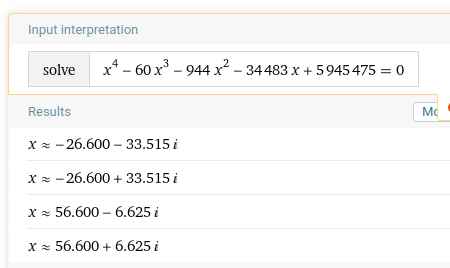
\includegraphics[scale=0.5]{roots_lab07_4d.png}
\]

\section{Выводы}

\tabС помощью степенного метода мы нашли максимальные по модулю комплексные собственные значения и соответствующие им собственные вектора. Использовали отделение корней, с помощью метода Ньютона решили уравнение $P^{\prime}(\lambda) = 0$

\end{document}

